\chapter[Multiple Culture Annotation]{Multiple Culture Annotation}
\label{ChapterAnnotation}

\thesiscomment{MAIN POINT: Because cultural perception differences are expected to exist, we collect a new cross culture annotation set using crowd sourcing and address the filtering issues to produce three distinct annotation sets that reflect individual annotator's ratings.}

\section{Introduction}

\thesiscomment{WHAT we do}

\thesiscomment{HOW we do it}

\thesiscomment{RESULTS, IMPACT and NOVELTY}

\thesiscomment{Of course, we expect to find cultural differences. Make it clear why this work is necessary despite that.}

This chapters describes the collection of \ac{NVC} annotations that are from culturally distinct sets of annotators. The previous two chapters describe an automatic system that attempts to recognises \ac{NVC} as humans would rate the same signal. This is complicated by the fact that humans often disagree as to what meaning has been expressed. One of the factors that affects \ac{NVC} signal perception by humans is the cultural background of the observer (see Section \ref{BackgroundWhatFactorsInfluenceNvc}). We address the need to recognise \ac{NVC} in a similar fashion to humans but using multiple groups of annotations, each which produce an independent subjective set of annotations. An automatic system can then better model the specific cultural perception of \ac{NVC} signals, which is an improvement compared to training a system in one culture and applying it in another culture that is not reflected in the training data.

All previous research has either gathered annotation data from a specific culture or merged annotations from multiple culture. This is the first study using subjective annotation used for machine learning when the cultures were kept as distinct annotation sets. However, this is not the first to use machine learning on subjective data with multiple groups of annotators. Reidsma and op den Akker, 2008 \cite{Reidsma2008b} trained classifiers on subjective annotations of contextual addressing in a meeting social context. As discussed in Section \ref{SectionAnalysisOfMeanRatings}, we have previously used the statistical mean of ratings to form a single label for each video clip. However, if there are significant inter-annotator disagreements in the data, taking the mean is not valid because the resulting label does not correspond to any specific human or group of human annotations.

The main contributions of this chapter are:
\begin{itemize}
 \item Perhaps the first use of crowd sourced data that is suitable for training and testing systems for automatic recognition of human behaviour.
 \item A method of filtering crowd sourced data to remove uncooperative workers.
 \item A quantitative analysis of cross cultural \ac{NVC} annotation data. This confirms that some perceptual cultural differences exist.
\end{itemize}

Research relating to cultural differences and crowd sourcing is discussed in the next section. Section \ref{SectionCrowdSourceDataCollection} describes the Internet based collection of annotation data. This data is filtered to remove uncooperative workers; the filtering method is described in Section \ref{SectionNeedToFilter}. Section \ref{SectionAnalysisOfCultureAnnotation} examines the resulting data to determine what cultural differences may exist.

\section{Related Research}
\label{BackgroundCrossCulture}

While there have been a vast number of cross cultural studies of human behaviour, none have been used as a basis for machine learning of cross cultural human behaviour recognition.

The field of cross cultural study of emotion was effectively founded by Darwin in 1872 \cite{Darwin2002}, in which he was struck by the remarkable similarity in emotion expression styles across cultures. His impact was later assessed by Ekman \cite{Ekman2009}, also very influential in the field of cross cultural emotion, who claimed that Darwin's key contributions were the emphasis of emotions that were discrete entities that were primarily expressed by the face and had partial universality across cultures and species. Darwin also pioneered the use of photographs in the study of emotion, and the assessment of emotion by judgment based studies which is now used by all annotator based emotion labeling systems. The key role of cultural effects in non-verbal communication was stressed by Hall \cite{Hall1959}, with particular attention to cultural influences that the expressor is not consciously aware. Ekman modeled the process of differences emotion expression by proposing culturally specific display rules \cite{Ekman1969}, but claimed that emotion subset was common to all cultures and termed these ``basic emotions'' \cite{Ekman1972}, although he also uses the term ``basic emotions'' for his particular discrete emotion/evolutionary view of emotions \cite{Ekman99}. There is less evidence for the universality of non-verbal communication but emotion can be a form of communication \cite{Frith2009}, so at least that component of \ac{NVC} as partially universal. Cultural differences exist for both expression and perception of emotion. Experimental work that examines these differences will now be discussed.

\thesiscomment{DISCUSS work in: expression differences and perception differences \cite{Matsumoto2006}}

% Possibly relevant? definition of basic emotions? \cite{Ortony1988}, 
Cultural differences in expression of emotion and \ac{NVC} have been observed. Gaze aversion while thinking has cultural differences \cite{McCarthy2006}. Different head motions are used for agreement and disagreement have been observed \cite{Kassabova2008}, as well as cultural differences in obscene gestures \cite{Knapp2009}. These differences may be significant for an automatic system if it is trained for one culture and deployed in a different culture. Various cross cultural studies have collected observer judgments and finding cultural differences each time. This has included judgments of pictograms \cite{Cho2007}, photographs \cite{Matsumoto08} and emotional avatars \cite{Massaro96} \cite{Koda2007}. Marsh \etal found that observes could distinguish a person's nationality by their style of emotional expression \cite{Marsh2003}. Japanese observers were found to be more sensitive to context than Westerners in emotion recognition \cite{Masuda2008}. Some universality was found for non-verbal vocalisation perception for the original Ekman 6 basic emotions but cultural differences were found in non basic emotions \cite{Sauter2009}. The process of perception has also been seen to have cultural differences: gaze patterns during emotion recognition were found to have culturally different patterns \cite{Jack2009}, which possibly lead to some cultures having difficulty distinguishing certain emotions. All these findings suggest that differences in expression and perception exist but also there is a great deal of commonality between cultures.

\thesiscomment{Any more perception papers?}

%A cross cultural study linked differences in display rule differences to cultural traits \cite{Matsumoto08}

Elfenbein and Ambady \cite{Elfenbein2002b} \cite{Elfenbein2002} argued that members of a cultural group are more accurate at recognising emotions in their group, when compared to an out of group observer. Matsumoto argued we cannot conclude that the in group hypothesis is true because of the lack of balancing the sample sizes and making the stimuli equivalent \cite{Matsumoto2006}. The potential for culturally specific concepts can make \ac{NVC} and emotion words difficult to translate or transfer to new cultures (see Section \ref{SectionTranslationOfInstrument}). If an in group advantage exists for \ac{NVC}, cultures that differ from the expressor's culture may annotate data differently. This may manifest itself as a reduction in inter-annotator agreement or misinterpretations of the \ac{NVC} meaning. 
% This may be that certain concepts are only meaningful within a culture (an ``emic'' account), which contrasts with an observer outside a culture that (an ``etic'' account) \cite{Headland1990}.

\thesiscomment{DISCUSS? Interannotator disagreements imply bad automatic results? \cite{Reidsma2008Thesis}}

\subsection{Crowd Sourcing of Annotation Data}

Crowd sourcing refers to the participation of a loosly defined group of people who work towards a common goal, often using the Internet to coordinate the work. Some scientific crowd sourcing projects have been very popular, with many workers from across the global, including Cooper \etal, \cite{Cooper2010} for ``foldit'' protein folding and Riddick \etal for ``Galaxy Zoo'' \cite{Raddick2010}. These projects generated enough public interest to not need payment to incentivise participation. Tarasov \etal \cite{Tarasov2010} proposed using crowdsourcing to gather emotional label annotation data. There are few or no previous works that use crowdsourcing for annotation of human behaviour, for the purposes of training an automatic recognition system. The next section describes how crowd sourcing was applied to annotation of \ac{NVC} samples.

\section{Data Collection Method}
\label{SectionCrowdSourceDataCollection}

We plan to collect annotation data from multiple cultures. The annotation task involves viewing a series of short views from the corpus (as described in Section \ref{SectionDescriptionOfTwoTalkCorpus}) and provide responses to the questions on \ac{NVC} signals (described in Section \ref{SectionDescribeQuestions}). Computer based annotation is very commonly used for corpus because the flexibility of the annotation tasks that may be defined and the convenience of collection and analysis of the results. Computer based annotation may also be conducted remotely, which is cost effective and convenience but provides less control on how the annotators complete the task. Differences in the equipment, the presence or absence of audio and a different physical environment may affect how an annotator perceives an \ac{NVC} signal. These factors could not be controlled using remote computer based annotation and may result in some inter-annotator differences.

Some tasks are sufficiently interesting as to not require a monetary incentive for annotators to participate. However, given our annotation task is relatively arduous (see Section \ref{BackgroundWhyNvcAnnotationIsBoring}), we opted to use Internet crowd sourced workers that were paid a small fee to complete each annotation task. Crowd sourced workers may be located anywhere in the world and use a standard web browser to complete tasks that have been defined by a work supplier. There is usually very little screening of workers and no qualification or requirements beyond being able to access the Internet. A typical screen shot of the web page presented to the annotator is shown in Figure \ref{FigureAnnotationSurveyScreenshot}. Although it is quite possible to establish a website that manages the web pages and payments, several web-based services manage this for a fee. We used Crowdflower's web service \footnote{\scriptsize{http://crowdflower.com/}} to manage our annotation work. This service provides a high level interface to other crowd sourcing services, such as Amazon Mechanical Turk \footnote{\scriptsize{https://www.mturk.com/}} and Samasource \footnote{\scriptsize{http://samasource.org/}}. Each worker pool has a distinct worker demographic and will be discussed later. However, crowd sourcing has several issues that need consideration if high quality annotation is required.

As previously mentioned, the order of the questions presented to the annotators is randomised to reduce the possible effect of question order on the results. During the annotation was being performed, it was impossible to insert a demographic survey before the users undertook the main task. This is unfortunate, because demographic information may be useful in quantifying  inter-annotator differences. However, the IP address of each annotator was provided, which can be used to assign a rough location of an Internet user. Also, Samasource specialises in refugee populations and an annotators current location can differ from their cultural background. In particular, we received a significant response from annotators located in Kenya, but these people were likely to be Sudanese refugees. Also, an IP address is not an absolutely reliable method, given the existence of internet proxy services. Despite these factors, IP addressed based locations was considered sufficient for our needs. In the case of refugees, we do not necessarily need to know the exact culture of origin, as long as the IP address location data results in multiple distinct cultural groups. Also, we may be sampling from only a sub-group within each culture. We use computer based tools to perform the annotation. The availability of skills and equipment availability varies for each population, therefore if we require computer skills for the participants, we will likely experience some sample bias. The extent of this bias is unknown. It may therefore be undesirable to sample from an entire country's population if the annotations within a group are not homogenous with respect to \ac{NVC} perception. However, we may be satisfied with a sub-group inside each of the cultures, while remembering the sample might not represent the culture as a whole. If we consider potential applications are likely to be adopted by segments of a culture which have easy access to technology, this bias may be beneficial in creating a system that operates well with potential computer literate users.

Our previous survey data was collected using unpaid volunteers (see Section \ref{SectionAnalysisOfHumanAnnotation}). This chapter uses paid workers to provide annotation data. Given that it was possible for an annotator to respond with random data in return for a monetary reward, there can be quality control issues which need to be managed. The process for separating valid work from random annotation data is described in Section \ref{SectionNeedToFilter}. We refer to workers that cooperate with the task as ``trusted'' workers, and annotators that respond with poor data or random data as ``untrusted''. Crowdflower provides it's own semi-automatic system for identifying trusted workers called ``gold'', presumably from the term ``gold standard''. This gold system was used to reduce the waste of money on poor annotation data. However, this gold system did not affect the final annotation data and both trusted and untrusted data was retained and filtered using the method we describe below.

\thesiscomment{Can a simple test question find random responders? Is this better than filtering?}

An alternative approach is identifying trusted workers is to introduce additional validation questions with predetermined answers that are used to determine if a worker should be trusted. Unfortunately, there are several practical reasons why this would not be effective in a crowd source application. Additional questions increase the amount of work required of the annotators. Because of current technical limitations of the annotation service, each annotation task or ``work unit'' must have the same number of responses for every question. The basic work unit requires the four \ac{NVC} signal ratings in our questionnaire. To add one more question per video would increase the annotator workload by 25\%. Also, humans that intend to cheat will be able to identify any validation questions and simply answer them currently with relatively little effort, while randomly answering the \ac{NVC} questions. This possibility of circumventing the validation questions makes their usefulness questionable. The results would still need to be analysed and filtered to provide confidence that the annotation data is valid.

Different languages are spoken throughout the world with English being the first language for approximately 380 million people \cite{Economist2001}. Second language speakers and learners of English outnumber first language users but the majority of people speak languages other than English. The next section discusses the issue of language in the context of \ac{NVC} signal perception ratings.

\subsection{Translation of Cross Cultural Instruments}
\label{SectionTranslationOfInstrument}

The design of the questionnaire was previously discussed in Section \ref{SectionDescribeQuestions}. Previously, we have only considered its use in a single culture and a single language. We intend to apply the questionnaire to cultures which have significant differences, including language usage. The translation of survey instruments is used in many scientific fields because the instrument may be understood is a different fashion outside of its original culture. According to Geisinger \cite{Geisinger1994}, we need to determine if an instrument needs to be translated and if a translated instrument measures the same constructs as the original version. A translation may lead to the instrument measuring something other than what was intended \cite{Poyatos1997}, and this makes comparison between cultures problematic. Translation of survey instruments is strongly recommended in medical surveys, using rigorous methods (\cite{Gjersing2010}, \cite{Beaton2000}, \cite{Morales2001}. Medical surveys contain questions that refer to concepts that are labels for observable phenomena that exist separately from the observer. However, our \ac{NVC} questionnaire is quite different in that the concepts that do not exist except as subjective interpretations. The questionnaire asks for an annotator's interpretation of \ac{NVC} signals which depends, to some extent, on their cultural background, and other factors. The very term ``\ac{NVC}'' implies that these communication signals do not directly correspond to word based concepts. De Mendoza \cite{Mendoza2008} argues emotion labels we use to express subjective interpretations are not ``defined by necessary and sufficient features'' but rather ``probabilistic concepts with an internal structure with better and worse examples of the category and fuzzy boundaries''. In this view, an emotion can be perceived as mostly agreeing, somewhat blaming, slightly surprised or any other combination of overlapping fuzzy labels. The same can be said of \ac{NVC} signal perception, in that the labels used in the questionnaire interrelated, fuzzy, partly overlapping and not comprehensive.

% Fernandez-Dols2003 discusses affect to get away from the realism/nominalism problem
% \cite{Davaninezhad2009}
% Translation of survey \cite{Ekman1969} \cite{Haralick1989} \cite{Headland1990} \cite{Marin1991} \cite{Humphrey1993} \cite{Geisinger1994} \cite{Poyatos1997} \cite{Morales2001} \cite{Economist2001} \cite{Fernandez-Dols2003} \cite{Thirumalai2003} \cite{Matsumoto2006} \cite{Cho2007} \cite{Mendoza2008} \cite{Davaninezhad2009} \cite{Gjersing2010} \cite{Noproblem}

If we use an instrument in multiple cultures, the concepts referred to in the instrument ideally would be consistently understood. There are two approaches that were considered: translating a questionnaire to cultures of interest or to present a single questionnaire in multiple cultures. These approaches will now be discussed in more detail.

If the concepts used in the questionnaire exist only in the mind of an observer, these concepts can be considered as cultural concepts and they do not necessarily exist in another language or culture. Because no one-to-one mapping exists between different cultural concepts, translation and cross culture recognition are problematic \cite{Elfenbein2002}. There are many examples of emotional concepts that do not have direct translations, such as translating \textit{verg\"{u}enza} from Spanish to English, \textit{shimcheong} from Korean to English \cite{Mendoza2008}. Applying this observation to \ac{NVC}, a particular communication action may be perceived in Spain as some combination of cultural concepts but in the United Kingdom, a different combination of cultural concepts. A perfect one-to-one mapping for translating culturally specific concepts might not exist. Cultural differences could therefore be cause by imperfect translation, leading to different the cultural concepts used by the annotation questions.

The other approach is to present the same single language questionnaire in multiple cultures. Because the words in the questionnaire would be interpreted by the annotators using their own cultural concepts, this will change the basis by which an annotator perceives \ac{NVC} signals. Cultural differences could therefore cause language understanding differences leading to different cultural concepts being used by the annotators.

Given both approaches have problems, we selected the second option of having a single survey in one language presented to all cultures. This decision was based on the fact that, given the crowd sourcing tools available at the time, a specific group of annotators could not be targeted by a tailored questionnaire, although this was planned for a future version of the service. Also, it may be possible to create a questionnaire using word coulds that would lend themselves better to probabilistic translation (e.g. mapping an English word cloud to Spanish word cloud). Given all these considerations, the transfer of everyday concepts from one culture to another is a complex issue and a subject worthy of further study. The next section takes the collected annotation data and considers how untrusted annotators can be identified and removed.

\section{Filter Untrusted Workers}
\label{SectionNeedToFilter}

\thesisstatement{Internet worker annotation is noisy, but trusted workers can be found by filtering the data}

\begin{figure}
\centering
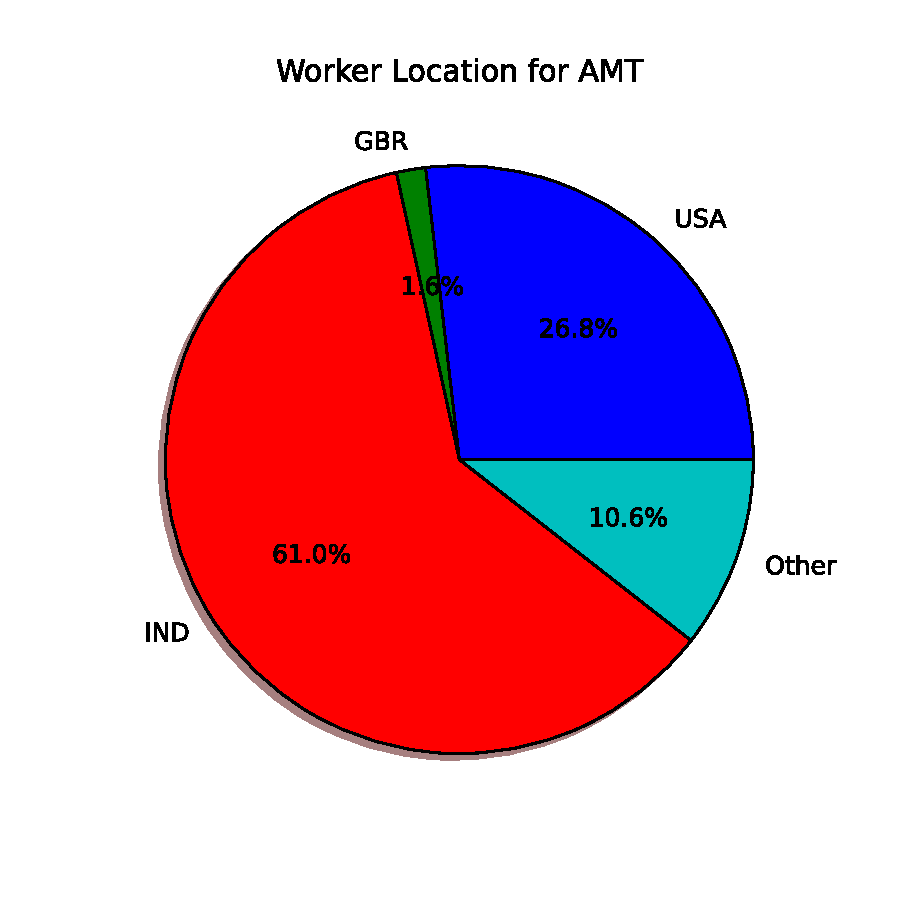
\includegraphics[width = 0.32 \columnwidth]{annotation/demog-amt.pdf}
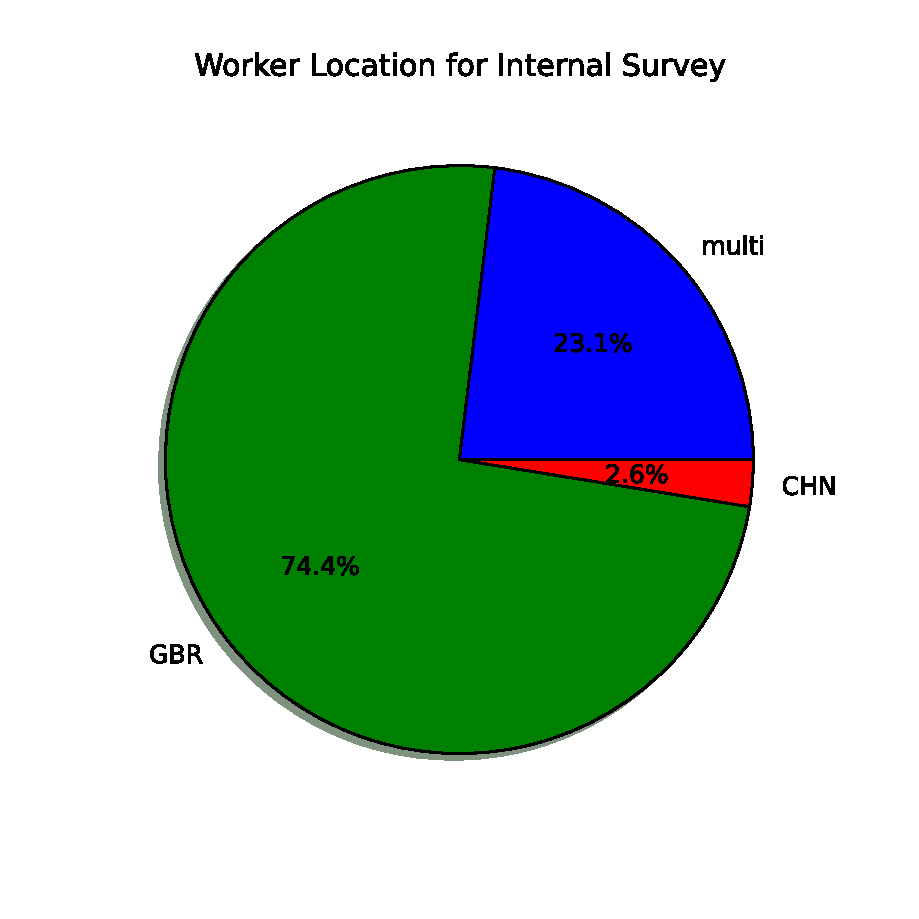
\includegraphics[width = 0.32 \columnwidth]{annotation/demog-internal.pdf}
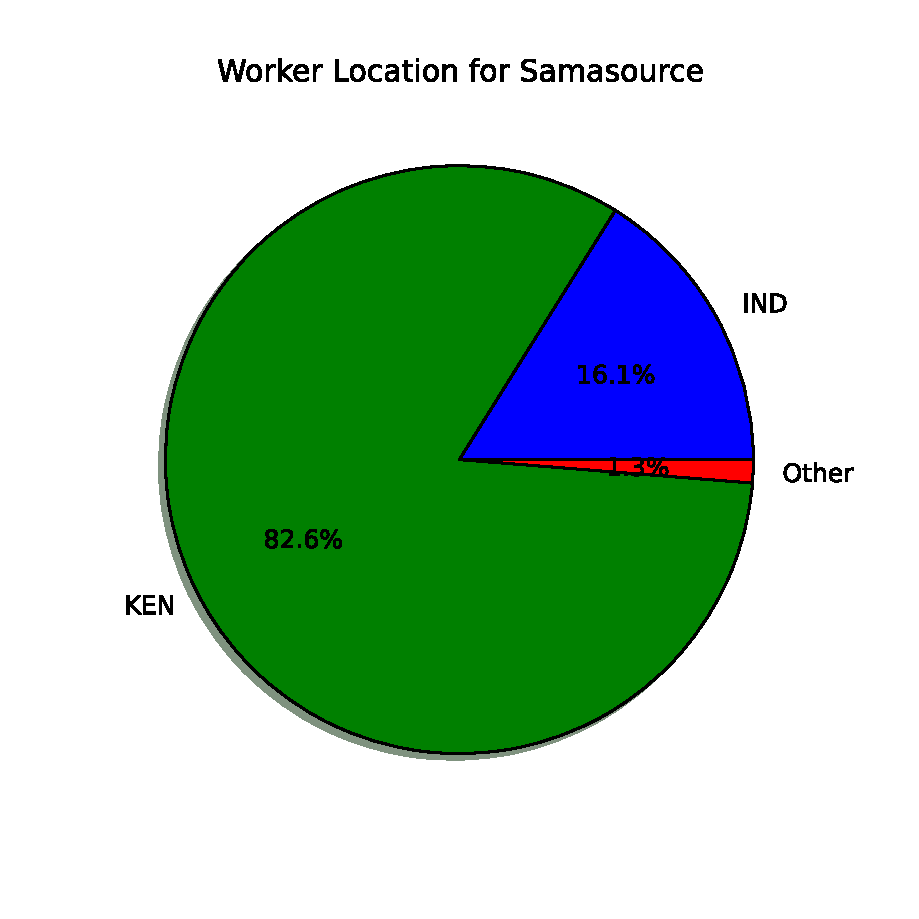
\includegraphics[width = 0.32 \columnwidth]{annotation/demog-sama.pdf}
\caption{Demographics of the worker pools. AMT is Amazon Mechanical Turk. Each country has been abbreviated to its ISO 3166 code. GBR Great Britain, KEN Kenya, IND India, USA United States of America.}
\label{FigureCrowdDemographics}
\end{figure}

The data collection method described in the previous section was used and resulted in 711 participants providing 79130 individual ratings. These ratings were distributed over 527 video clips and 4 \ac{NVC} categories, with a total of $527 \times 4 = 2108$ questions. However, a significant proportion of the annotation data was of poor quality or random, due to a significant proportion of uncooperative annotators. In all, annotators from 33 countries participated in the annotation task. As discussed, three worker pools were used. As can be seen in Figure \ref{FigureCrowdDemographics}, the demographics of each pool differ quite dramatically. Because the annotation data for a single annotator is usually sparse (meaning they are not required to complete every question in the survey), we require a significant amount of annotation from a culture before there is sufficient to have multiple votes on every question in the survey. A significant amount of annotation data was received from GBR (Great Britain), KEN (Kenya) and IND (India) and these three cultures are used throughout the remainder of this thesis. The data from annotators based in other cultures was discarded, because each annotator did not complete enough questions to have a complete result set. With better targeting of annotation resources, it would be possible to greatly increase the number of distinct cultures.

If the data is not filtered, the resultant labels are extremely noisy and are not appropriate for machine learning. Given data from each culture, we divide workers into trusted and untrusted groups depending on their cooperation with the task. The next section describes the filter method used to ensure the labels are of sufficient quality.

\subsection{Filtering Method}
\label{SectionAnnotationFilterMethod}

\begin{figure}
\centering
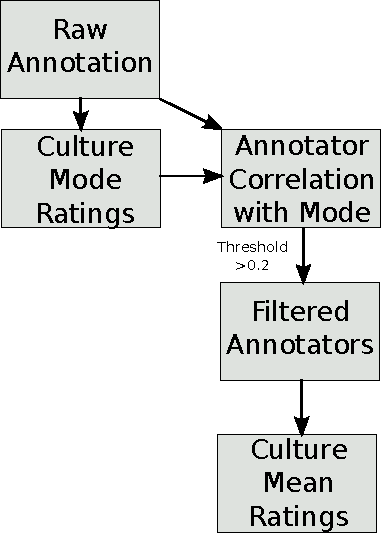
\includegraphics[width = 0.3 \columnwidth]{annotation/FlowAnnotationFiltering.pdf}
\caption{Flow chart of filtering method. The statistical mode rating provides a robust standard by which annotators are assigned a trusted or untrusted score.}
\label{FigureFilterFlowChart}
\end{figure}

As discussed, we have three cultures of interest: GBR, IND and KEN. The aim is to split annotators into two groups: trusted and untrusted. To achieve this, each worker's data $\rawAnnotation_i$ is compared to a robust rating standard $\robustAnnotation$. If a worker correlates with the robust standard to a sufficient degree, they are assigned to the trusted group and if not, the untrusted group (see Figure \ref{FigureFilterFlowChart}). The robust rating standard is based on the rating mode for clip $\clipId$, \ac{NVC} category $\nvcCategory$:

\begin{gather}
\robustAnnotation^{\clipId}_{\nvcCategory} = mode(\rawAnnotation^{\clipId}_{\nvcCategory})
\end{gather}

\begin{figure}
\centering
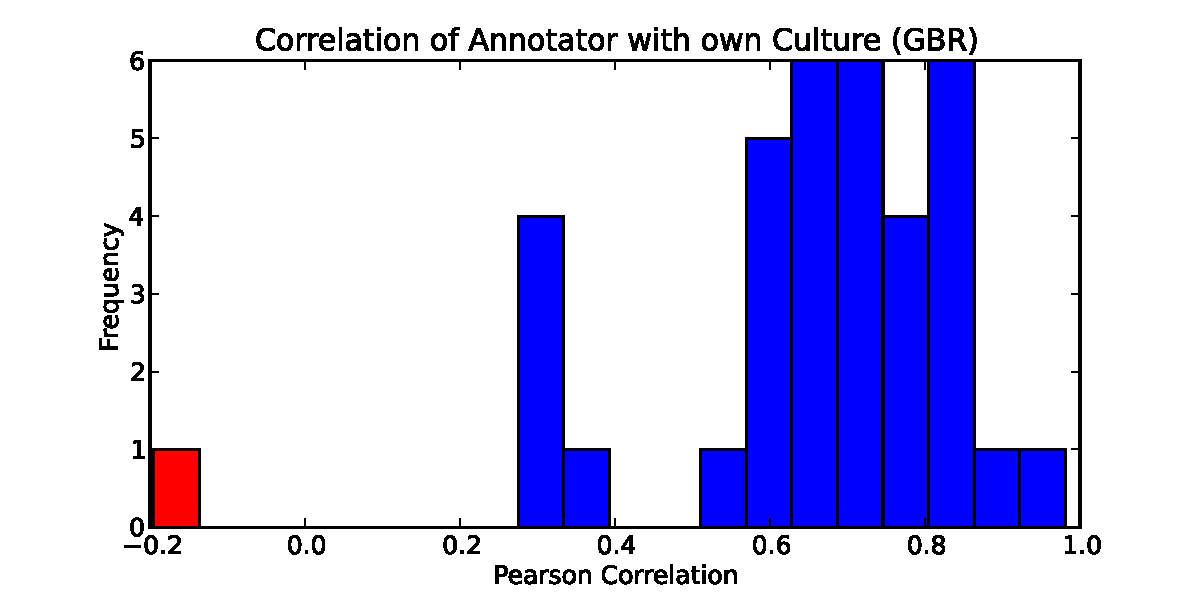
\includegraphics[width = 0.6 \columnwidth]{annotation/correlgbr.pdf}
\caption{Histogram of annotator correlation $\rho$ for GBR when compared to the robust ratings $\robustAnnotation$. Blue bars indicate annotators above the trusted threshold $\trustedThreshold$, and red bars indicate workers below. The majority of annotators in the GBR have relatively good agreement with the robust rating.}
\label{FigureCorrelationHistOfGbr}
\end{figure}

\begin{figure}
\centering
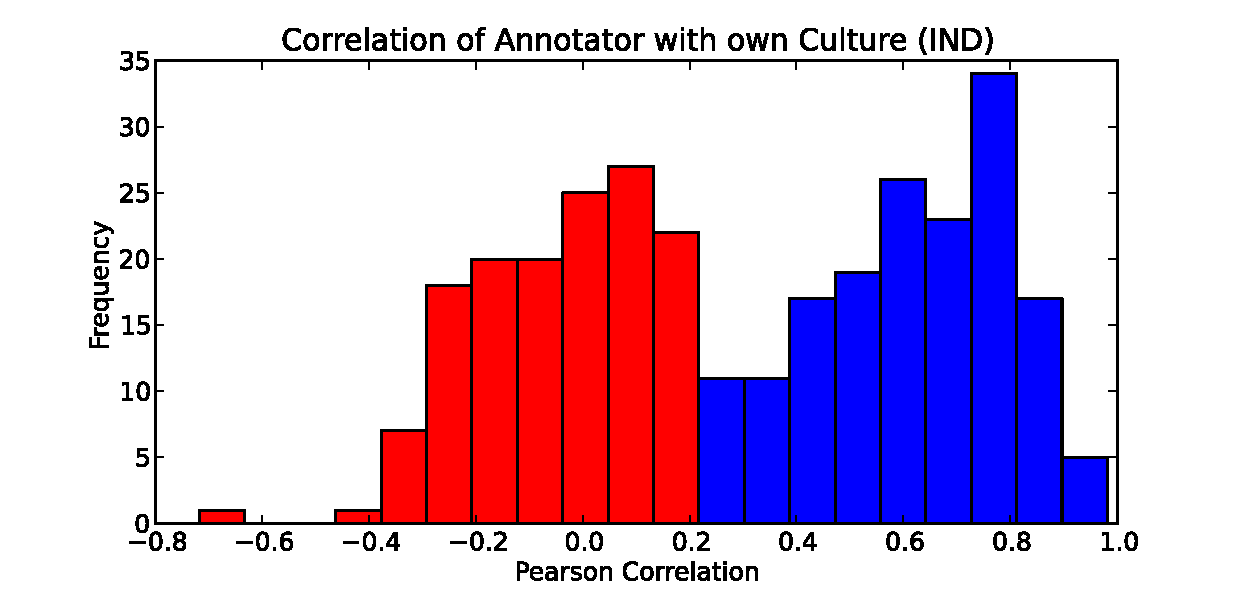
\includegraphics[width = 0.6 \columnwidth]{annotation/correlind.pdf}
\caption{Histogram of annotator correlation $\rho$ for IND when compared to the robust ratings $\robustAnnotation$. Blue bars indicate annotators above the trusted threshold $\trustedThreshold$, and red bars indicate workers below. A significant number of workers in the IND group were assigned to the untrusted group.}
\label{FigureCorrelationHistOfInd}
\end{figure}

\begin{figure}
\centering
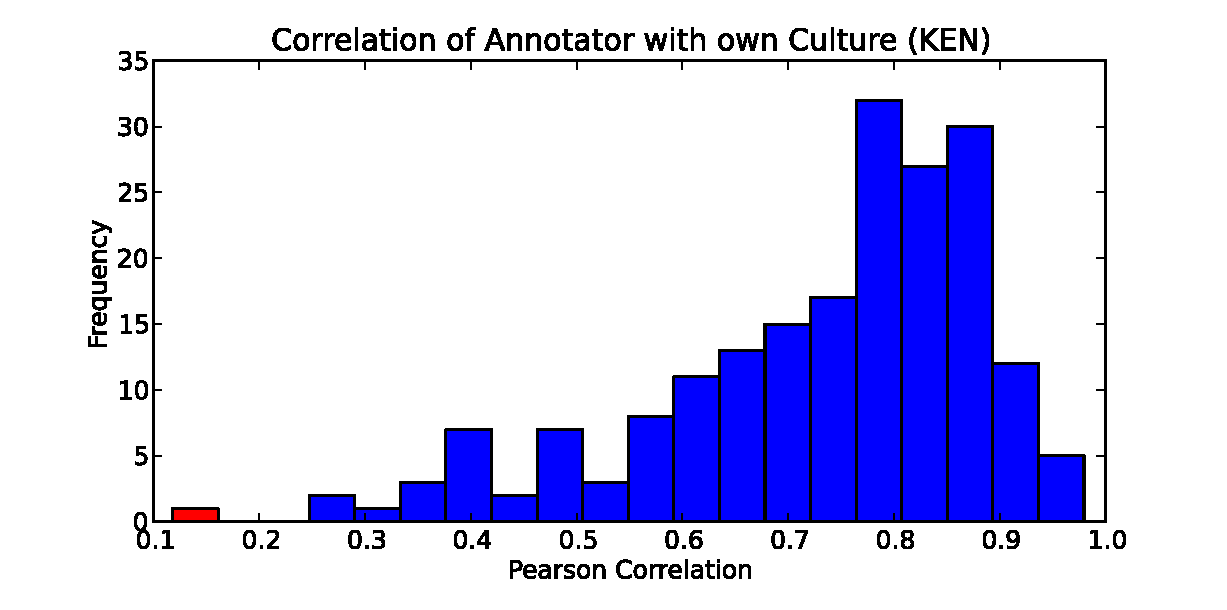
\includegraphics[width = 0.6 \columnwidth]{annotation/correlken.pdf}
\caption{Histogram of annotator correlation $\rho$ for KEN when compared to the robust ratings $\robustAnnotation$. Blue bars indicate annotators above the trusted threshold $\trustedThreshold$, and red bars indicate workers below. The majority of annotators in the KEN have relatively good agreement with the robust rating.}
\label{FigureCorrelationHistOfKen}
\end{figure}

The statistical mode is used because it is relatively robust to uniformly distributed noise give a sufficient quantity of samples. Note that we normally consider $\rawAnnotation$ as a continuous variable but here we consider it as a quantised variable. This is possible because the annotator responses used a Likert scale with a finite number of options. Histograms of annotator correlation from the three cultures of interest are shown in Figures \ref{FigureCorrelationHistOfGbr}, \ref{FigureCorrelationHistOfInd} and \ref{FigureCorrelationHistOfKen}. As can be seen, there are cultural differences in the proportion of annotators assigned to the trusted and untrusted groups. IND had a significant proportion of untrusted workers, while GBR and KEN annotators were largely assigned to the trusted group. These differences in trust are probably associated with the crowd sourcing worker pools, in particular their recruitment and worker screening policy, rather than a cultural difference. The vast majority of untrusted workers were from the Amazon Mechanical Turk pool, while annotators from the Samasource and Internal pools were largely trusted. Each annotator $i$ is compared to the robust standard $\robustAnnotation$ using Pearson correlation coefficient $\rho$:

\begin{gather}
\rho_i = correl(\rawAnnotation_i,\robustAnnotation_i) \\
i \in \begin{cases}
trusted : \rho_i \ge \trustedThreshold \\
untrusted : \rho_i < \trustedThreshold
\end{cases}
\end{gather}

If an $i$ annotator's correlation $\rho_i$ is above the trusted threshold $\trustedThreshold$, it is included in the set of trusted annotators. The final filtered annotation $\filteredAnnotation$ by taking the statistical mean of trusted annotators.  The mean is used rather than the mode because the mode only considers the peak of this distribution but disregards the other samples. However, considering the entire distribution with the mean is more sensitive to the overall views of the annotators. The mean does not suffer information loss from being a discretised variable. However, the mean is not a robust measure, which is why it is applied after the data is filtered.

\begin{gather}
\filteredAnnotation^{\clipId}_{\nvcCategory} = mean(\rawAnnotation^{\clipId}_{\nvcCategory,i}), i \in trusted
\end{gather}

%\begin{table}
%\centering
%\caption{Number of annotators and votes for cultures included in the unfiltered and filtered $\filteredAnnotation$ data set.}
%\begin{tabular}{ | c | c  c | c  c | }
%\hline
%Annotator & \multicolumn{2}{c|}{Num. Annotators} & \multicolumn{2}{c|}{Num. Ratings}  \\
%Country & Unfilter & Filter & Unfilter & Filter \\
%\hline
%\hline
%India & 304 & 167 & 37147 & 22754 \\
%Kenya & 196 & 195 & 15452 & 15420 \\
%GBR & 36 & 26 & 8211 & 8167 \\
%\hline
%\end{tabular}
%\label{NumFilteredWorkersTable}
%\end{table}

\begin{table}
\centering
\caption{Number of annotators and votes for cultures included in the unfiltered and filtered $\filteredAnnotation$ data set.}
\begin{tabular}{ | c || c | c  c || c | c  c | }
\hline
Annotator & \multicolumn{3}{c||}{Num. Annotators} & \multicolumn{3}{c|}{Num. Ratings}  \\
Country & Total & Trusted & Untrusted & Total & Trusted & Untrusted \\
\hline
\hline
India & 304 & 167 (55\%) & 137 & 37147 & 22754 & 14393\\
Kenya & 196 & 195 (99\%) & 1   & 15452 & 15420 & 32\\
GBR   & 36  & 26  (72\%) & 10  & 8211  & 8167  & 44\\
\hline
Total & 536 & 388 (72\%) & 358 (28\%) & 60810 & 46341 & 14469\\

\hline
\end{tabular}
\label{NumFilteredWorkersTable}
\end{table}

The quantity of annotations assigned to the unfiltered $\rawAnnotation$ and filtered $\filteredAnnotation$ annotation sets are shown in Table \ref{NumFilteredWorkersTable}. The 28\% of users that were assigned to the untrusted group accounted for 23\% of the unfiltered data. This implies the trusted annotators answered a greater number of questions on average. A significant amount of data is still available, after filtering, for use in training and evaluating machine learning techniques. Each annotator is associated with a single culture. In summary, a culturally specific robust ratings set is found ($\robustAnnotation_{GBR}$,$\robustAnnotation_{IND}$,$\robustAnnotation_{KEN}$), which are used to filter annotators to form a final, culture specific, filtered annotation ratings $\filteredAnnotation_{GBR}$, $\filteredAnnotation_{KEN}$ and $\filteredAnnotation_{IND}$.

\thesiscomment{Is consensus just an artifact of filtering? Hair colour?}

A method of finding a subset of trusted workers based on their mutual agreement has been described. Given that untrusted annotators tend to provide uniformly random responses, we will expect that the variance of ratings is lower in the filtered set $\filteredAnnotation$ when compared to the unfiltered data $\rawAnnotation$. There is an theoretical possibility that a minority of self consistent annotators might be selected while the trusted set might not represent an overall consensus. However, Table \ref{NumFilteredWorkersTable} shows that the majority of annotators are retained in the trusted set, which indicates a small subset of annotators has not been selected over a broader valid set.

Given the filtered data $\filteredAnnotation_{GBR}$, $\filteredAnnotation_{KEN}$ and $\filteredAnnotation_{IND}$, cultural differences between the annotators can be analysed. This is discussed in the following section.

\section{Analysis of Annotations}
\label{SectionAnalysisOfCultureAnnotation}

The previous section has described how annotation data was collected from Internet workers and applied filtering to obtain a high quality set of \ac{NVC} annotations. This annotation data describes the \ac{NVC} content for either \textit{agree}, \textit{thinking}, \textit{question} or \textit{understand} as observed from a particular culture (GBR, KEN or IND). However it is well known that \ac{NVC} perception is dependent on cultural rules. The specifics of cultural influences on \ac{NVC} perception are not well understood. This section provides a quantitative analysis as to the extent of the cultural differences.

\thesisstatement{Annotation of NVC has a low inter-annotator agreement}

\thesisstatement{Different cultures have distinct patterns in their annotation results}

%$\rho_{IND,KEN} = correl(\filteredAnnotation_{IND},\filteredAnnotation_{KEN})$
\begin{table}
\centering
\caption{Inter-culture correlation of filtered data for different culture pairs.}
\begin{tabular}{ | c | c c c | }
\hline
 & India & Kenya & GBR \\
\hline
\hline
India & 1 & 0.56 & 0.55\\
Kenya &  & 1 & 0.64 \\
GBR    &  &  & 1 \\
\hline
\end{tabular}
\label{InterCultureCorrelationTable}
\end{table}

As can be seen in Table \ref{InterCultureCorrelationTable}, the correlation of pairs of cultures is at an intermediate level. We might expect to see a correlation less than one (perfect correlation), because previous studies of emotion have observed cultural differences (see Section \ref{BackgroundWhatFactorsInfluenceNvc}). Also, we have already discussed possible causes for culture differences in annotation in Section \ref{SectionTranslationOfInstrument}. A correlation above zero (no correlation) means \ac{NVC} perception in different cultures is not totally independent and some commonality exists. This confirms our suspicion that \ac{NVC} perception is similar to emotion perception in that cultural differences exist, but there remains significant commonality between cultures. Another point that is illustrated by Table \ref{InterCultureCorrelationTable} is that some cultures are more similar to others in perception of \ac{NVC}. The KEN-GBR correlation is higher than either IND-GBR or IND-KEN ($0.64$ vs. $0.56$ or $0.55$). This suggests that IND is the most distinctive in \ac{NVC} perception, and KEN-GBR are relatively similar. It might be expected that other pairs of cultures are much more or much less similar than the three cultures studied. We have restricted our work to areas with access to computer and Internet resources, but a wider examination of cultural differences would be interesting.

It should be noted that Pearson's correlation coefficient is insensitive scaling differences. This is a desirable property, because scaling differences between cultures are relatively trivial to understand and model. However, the less than perfect correlation scores indicate that annotation differences exist and that they are not merely linear scaling differences.

\begin{figure}
\centering
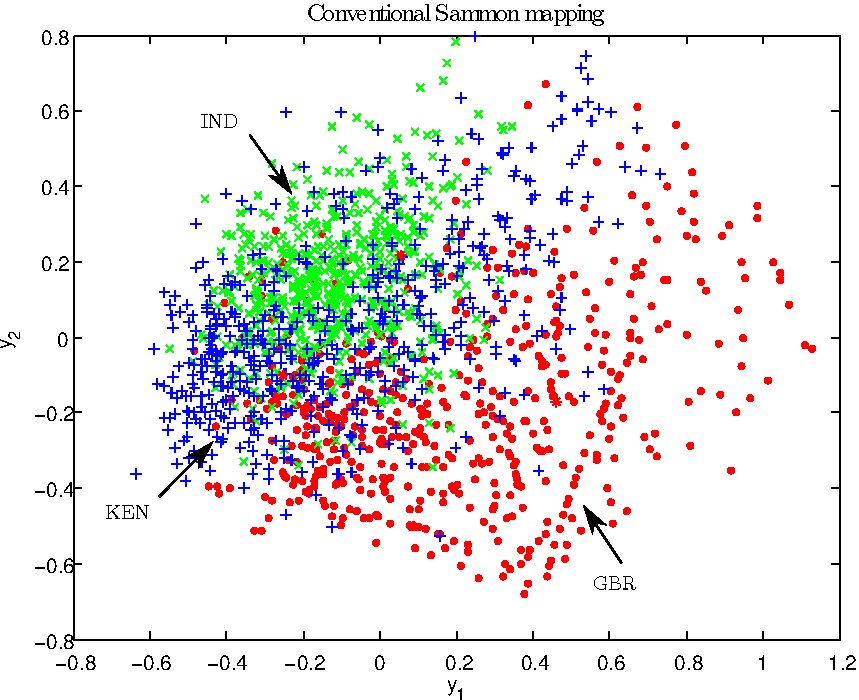
\includegraphics[width = 0.78 \columnwidth]{annotation/Sammon3Culture.pdf}
\caption{Sammon mapping of the filtered annotation responses. Each point represents the mean rating of a single clip within a single culture. The four \ac{NVC} categories are concatenated into a 4{D} vector to enable distance pairs to be computed.}
\label{CultureSammonMapping}
\end{figure}

A way of visualising cultural differences in annotation of \ac{NVC} perception is the Sammon mapping \cite{Sammon1969}. This technique is a dimensional reduction tool to map high dimensional samples to a lower dimensional space while preserving inter-sample distances. Each filtered culture annotation $\filteredAnnotation$ is a $527$ by $4$ matrix. We combine the three filtered cultures (GBR, IND, KEN) into a $3 \times 527$ by $4$ matrix, then reduce this to a 2{D} space using Sammon mapping and plot the sample positions. This allows us to visualise and compare the distribution of annotation responses for different cultures. The result of this procedure, shown in Figure \ref{CultureSammonMapping}, is a complex distribution with some regions that are generally exclusive to a single culture, other areas that are densely occupied by two overlapping cultures and one central zone where all cultures have a high density. The area of three culture overlap corresponds to annotation responses that appear in all cultures, the most common of which is most likely to mean ``no \ac{NVC} is being expressed''. Areas that are dominated by a single culture are interesting because they imply that for a subset of clips, a culture has provided a 4 category rating that does not appear in the other cultures. This seems to be most apparent in the GBR annotations which as a significant proportion of points that are very far from any other culture's points. This supports the idea that cultural differences in \ac{NVC} are not trivial to explain or model and may be highly non-linear when comparing one culture to another. 

\thesisstatement{People correlate better with their own culture consensus than with a global consensus}

\thesisstatement{Taking the global mean doesn't correspond to anything in real applications}

\begin{table}
\centering
\caption{Correlation of the mean annotator correlation within various cultures with their respective culture filtered annotation $\filteredAnnotation$ or the global Mean (taken as the combined India, Kenya and \ac{UK} ratings). Annotators correlate better on average with their own culture consensus than the global consensus $\globalAnnotation$.}
\begin{tabular}{ | c | c c c | }
\hline
 & India & Kenya & \ac{UK} \\
\hline
\hline
Own Culture Mean & 0.67 & 0.78 & 0.77 \\
Global Mean & 0.64 & 0.74 & 0.68 \\
\hline
\end{tabular}
\label{MeanAnnotatorCorrelationTable}
\end{table}

Because we used various filtering methods and mean ratings to arrive at the filtered annotations $\filteredAnnotation$, we need to check to what extent the filtered annotations are representative of the individual annotator responses. Also, we can see the effect if culture is ignored and the ratings are combined to produce a global mean $\globalAnnotation$.
%The filtered annotations is intended to represent the overall culture's \ac{NVC} perception and we should expect a annotator to be more similar to their respective culture, rather than a different culture. TESTS NOT DONE
These comparisons are shown in Table \ref{MeanAnnotatorCorrelationTable}. A person's correlation to their own culture is relatively good. The lower annotator to consensus score of IND may indicate a problem with data quality or perhaps there is greater perception individuality in that annotator group.
However, if cultural difference is ignored as in the case of global mean annotation $\globalAnnotation$, the individuals do not correlate as well in every culture. Therefore there is a divergence between individual annotators and the ratings that are intended to reflect them. Remember that taking a mean of individual ratings if the annotators form a relatively self-consistent group. Therefore, ignoring culture produces a global annotation that has less validity. If this were applied to a machine learning task, the labels that would be predicted would not necessarily correspond to any annotator or subset of annotators. This ignores one of the primary objectives of producing an automatic system that would predict \ac{NVC} as a human would perceive \ac{NVC} (see Section \ref{SectionClassificationIntro}).

\thesiscomment{TODO Tests that confirm individuals correlate with their own culture on average, rather than other cultures?}

\thesiscomment{DISCUSS differences exist other than culture and this is seen here, an area for further work}

\thesiscomment{DISCUSS When does the score converge? about 5 filtered votes?}

\thesiscomment{DISCUSS Any more ideas for analysis? Is there a way to map clusters from different cultures?}

Conclusions are drawn in the next section, based on the experience of collecting data annotation and the analysis results.

\section{Conclusion}

\thesiscomment{DISCUSS If we have much more data, we could use unsupervised clustering without needing demographics. Or demographics can assist in semi-supervised clustering.}

This chapter has described the collection of cross cultural communication perception annotation data. The data was collect from paid Internet workers from multiple cultures. Because of some workers not cooperating, the data was filtered to use only valid annotation data. The annotations were analysed and found to contain differences that are not merely linear scaling effects. This data annotation resulted in a new, cross cultural annotation of \ac{NVC} on natural informal conversations. The annotation data has been released for reuse. This helps to address the lack of publicly available \ac{NVC} annotation data. 

Crowd sourcing annotation data may prove to be a significant resource in human behaviour understanding if quality issues can be addressed. The quality assurance tools that are currently available are focused on annotation of objective labels. These objective labels are appropriate for computer vision tasks such as object recognition where the concepts are well defined. And example question for object recognition can be as simple as a binary choice ``Is there are car in this photograph?''. Any disagreement in annotators usually indicates that the minority view is incorrect, based on the assumption that untrusted workers provide random responses rather than trying to sabotage the annotation exercise. These filtering methods are not useful in subjective tasks, such as \ac{NVC}. In this case, inter-annotator differences do not necessarily imply that some of the annotators are wrong, due to perceptual differences. However, quality is still a significant concern and the filtering method proposed in this chapter is a step towards addressing this. The filtering method does rely on using the annotation mode, which depends on sufficient annotator participation to form a stable result. Also, the annotators are hard assigned to trusted and untrusted groups. It may be more efficient to use soft assignments for annotator trust.

The presence of cultural perception differences is not particularly surprising given this effect is often observed in emotion. What is significant about the findings of this chapter are the confirmation and a quantitative analysis of the differences. The results suggest that different culture pairs have varying degrees of similarity. These cultural similarities might be exploited to reduce the number of different culturally specific models needed for \ac{NVC} recognition, possibly by treating actual annotator group perceptions as a mixture of two or more exemplar perception models.

There are some significant shortcomings of Internet crowd sourcing for studying perception. The selection of annotators and the environment in which the annotation is performed is not controlled. Different cultures have different availability of computer resources, different levels of computer competency, different demographics that will undertake the task and different locations at which the annotation is performed. These differences are known to be a factor in emotion perception and are likely to play a role in \ac{NVC} perception. The use of demographic questions may allow some of these variables to be controlled. This chapter has used English language questionnaires, but there can be cultural differences in the understanding of language. Given that perception differences in this chapter may be caused by either language perception differences or \ac{NVC} perception differences, it is hard to distinguish these effects. One possible method to check and possibly quantify language differences in crowd source annotation is to conduct cross cultural annotation of data that has objective labels, using a single language questionnaire. If the annotators were consistent across cultures, this result would validate the general approach. Translation of \ac{NVC} survey instruments replaces the uncertainty of language perception with uncertainty over the validity of the translation of \ac{NVC} concepts, which by definition do not directly correspond to word based concepts.

%Emotion is studied by examining the response to an emotionally inducing stimuli. However, \ac{NVC} focuses on conscious action, rather than automatic reaction. It is possible that culturally equivalent stimuli do not exist for \ac{NVC}.

The next chapter uses this annotation data to approach the \ac{NVC} recognition problem by cross cultural regression. This is intended to better model cultural perception differences observed in this chapter.
